\section{Scheduling} \label{sc:scheduling}
In scheduling the aim is to meet all hard deadlines and handle soft deadlines of jobs in the best possible manner and avoid deadlocks while doing so. The arrival time of a job is the moment in time it arrives at a processor, while the release time of a job is the moment in time it becomes available for execution. A task can have different job types and such as periodic, sporadic and aperiodic. A task is a set of jobs known at the start of the system or triggered by a external event.

A periodic task is defined:
\begin{itemize}
	\itemsep0em
	\item The release time \textit{r} of the first periodic job.
	\item The period \textit{p}, which is a periodic time interval, at the start of which a periodic job is released.
	\item The execution time \textit{e} of each periodic job.
	\item The deadline \textit{d} of each periodic job.
\end{itemize}
and is written as $J_n=(r,p,e,d$)

\subsection{Rate-monotonic scheduler}
The rate-monotonic scheduling strategy gives a higher priority to periodic jobs with a shorter period. Because of the static nature of the scheduler, it is easy to compute and predict.\footnote{\cite[p.~183]{Fokkink1965}}
%--- This can be removed if we need space?
We define three periodic jobs: $J_1$ with a period of 20 and a execution time of 3, $J_2$ with a period of 5 and a execution time of 2, $J_3$ with a period of 10 and a execution time of 2. All with a release time of 0 and the deadlines are not defined. Figure \ref{fig:rateMonotonicExample} shows the execution of the three jobs using a rate-monotonic scheduler.
%---

\begin{figure}[!ht]
	\centering
	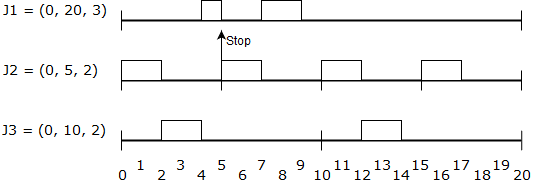
\includegraphics[scale=0.5]{realTimeComputing/fig/rate-mono.png}
	\caption{Example of rate-monotonic scheduling.}
	\label{fig:rateMonotonicExample}
\end{figure}

As can be seen on Figure \ref{fig:rateMonotonicExample}, the first job to be executed is $J_2$ followed by $J_3$. $J_1$ is then started but gets preempted by the scheduler, because $J_2$ starts a new execution on period 5. $J_2$ has a shorter period and therefore has a higher priority. $J_3$ continues execution after $J_1$.

\subsection{Earliest deadline first scheduler}
This scheduling strategy will give a higher priority to jobs if their deadline is
early. In case of preemptive jobs and no competition for resources, this scheduler
is optimal, in the sense that if utilization at a processor does not exceed one, then
periodic jobs will be scheduled in such a way that no deadlines are missed.\footnote{\cite[p.~184]{Fokkink1965}}

\begin{figure}[!ht]
	\centering
	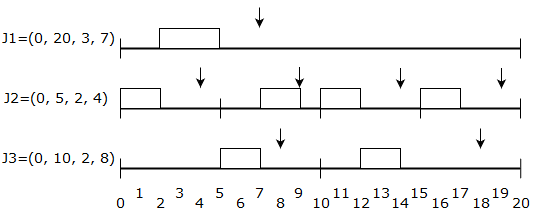
\includegraphics[scale=0.5]{realTimeComputing/fig/EarliestDeadlineFirst.png}
	\caption{Example of Earliest deadline first and Least-slacktime-first scheduler.}
	\label{fig:EarliestDeadlineFirstAndLeastSlacktimeFirstSchedulerExample}
\end{figure}

The example in Figure \ref{fig:EarliestDeadlineFirstAndLeastSlacktimeFirstSchedulerExample} can be viewed as using Earliest deadline first scheduler. This approach is dynamic meaning it evaluates the jobs each time unit. The first job to be executed is $J_2$ because it has earliest deadline followed by $J_1$ and $J_3$.

\subsection{Least-slacktime-first scheduler}
This scheduling strategy gives higher priority to jobs with less slack time (i.e. idle time). This scheduler is a good choice if utilization at a processor does not exceed one. In this case the periodic jobs will be scheduled in such a way that no deadlines are missed.\footnote{\cite[p.~184]{Fokkink1965}} We use the following formula to determine the slacktime: $L(T)=D(T)-C(T)$, Where $T$ represent the time, $L(T)$ represent the laxity (slack), $D(T)$ represent the time between the closest deadline and the current time, $C(T)$ represent the remaining time of execution. For each time-frame a calculation of all the processes are done and the one with the least slacktime will be prioritized.

The example in Figure \ref{fig:EarliestDeadlineFirstAndLeastSlacktimeFirstSchedulerExample} can be viewed as using Least-slack time-first scheduler. Note that it is a coincidence that both least-slacktime-first and deadline first schedulers act the same, for this example. At $T=0$ the three formulas will look as follows:
\begin{align}
	L_1(0)=7-3&=4 \\
	L_2(0)=4-2&=2 \\
	L_3(0)=8-2&=6
\end{align}
At $T=0$, $J_2$ has the least slack and is therefore prioritized. This procedure will be followed for every timeframe and the job with least slack will be prioritized. In case the slack of two jobs are the same (As at time $T=4$ and $T=6$, in this example), the process that is currently running will be prioritized.

\section{Resource control}

One of the pitfalls of sharing resources is deadlocks, as competing processes wanting the same resource could introduce race conditions\footnote{Race conditions: A race condition or race hazard is the behavior of an electronics, software, or other system where the output is dependent on the sequence or timing of other uncontrollable events.} resulting in the jobs blocking each other and often an unpredictable outcome. We consider a high priority Task H, a medium priority task M and a low priority Task L. When a phenomenon called priority inversion occurs, Task H is preempted by a lower priority task, causing the priorities to be inverted. This could occur if Task L is using some shared resource R in its critical section, Task H arrives requesting R, but gets blocked because it is in use by Task L. Now a Task M starts executing during Task L's use of R, and since Task H is blocked waiting for Task L, Task M is now the highest priority task in the system, so it occupies the processor without no task being able to preempt it. Task H is now at the bottom of the executing chain waiting for Task L that waits for Task M to finish. Figure \ref{fig:priorityinversion} shows this.  We will discuss two protocols that can remedy these issues named \textit{priority inheritance} and \textit{priority ceiling}.

\begin{figure}[!ht]
	\centering
	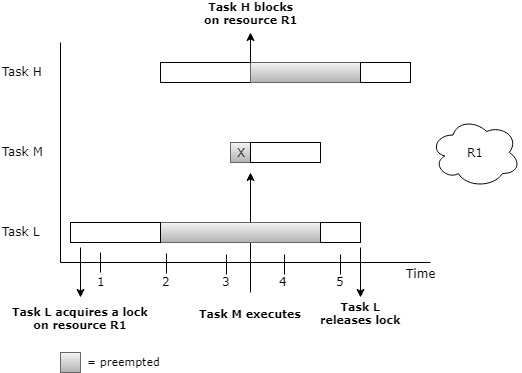
\includegraphics[scale=0.5]{realTimeComputing/fig/PriorityInversion.png}
	\caption{Priority inversion in action - Task H becomes the bottom of the executing chain.}
	\label{fig:priorityinversion}
\end{figure}

\subsection{Priority inheritance}

This protocol uses dynamic priority adjustments to change task priorities on the fly. Assume Task L is running and uses some shared resource. If Task H arrives and requests ownership of the same shared resource, Task L gets elevated to the priority of the requesting Task H. Task L would then continue executing its critical section. Once it is done, the task gets dropped down to its original priority, allowing Task H to take control of the resource. Priority inheritance makes it less likely that a high priority job gets blocked by the lower one, however each nested resource lock would increase the wait time for a pending task to complete. The maximum wait time would be the sum of all the execution times of all of the nested resource locks.

\subsection{Priority ceiling}

With priority ceiling all tasks that will access a given shared pool of resources are evaluated before executing and each resource is assigned a predefined priority based on the task with the highest priority that will access the resource. This is called a priority ceiling. When a task requires a resource, the task's priority is elevated to match that of the resource, ensuring that the task will not be preempted by any other task. Once it completes, the task is dropped down to its original priority. The maximum wait time for a high-priority task is limited to the longest critical section of any lower-priority task that accesses the shared resource.

